\documentclass[border=8pt]{standalone}
\usepackage{amsmath,amssymb,mathtools}
\usepackage{tikz}
\usetikzlibrary{arrows.meta,calc,positioning}
\begin{document}
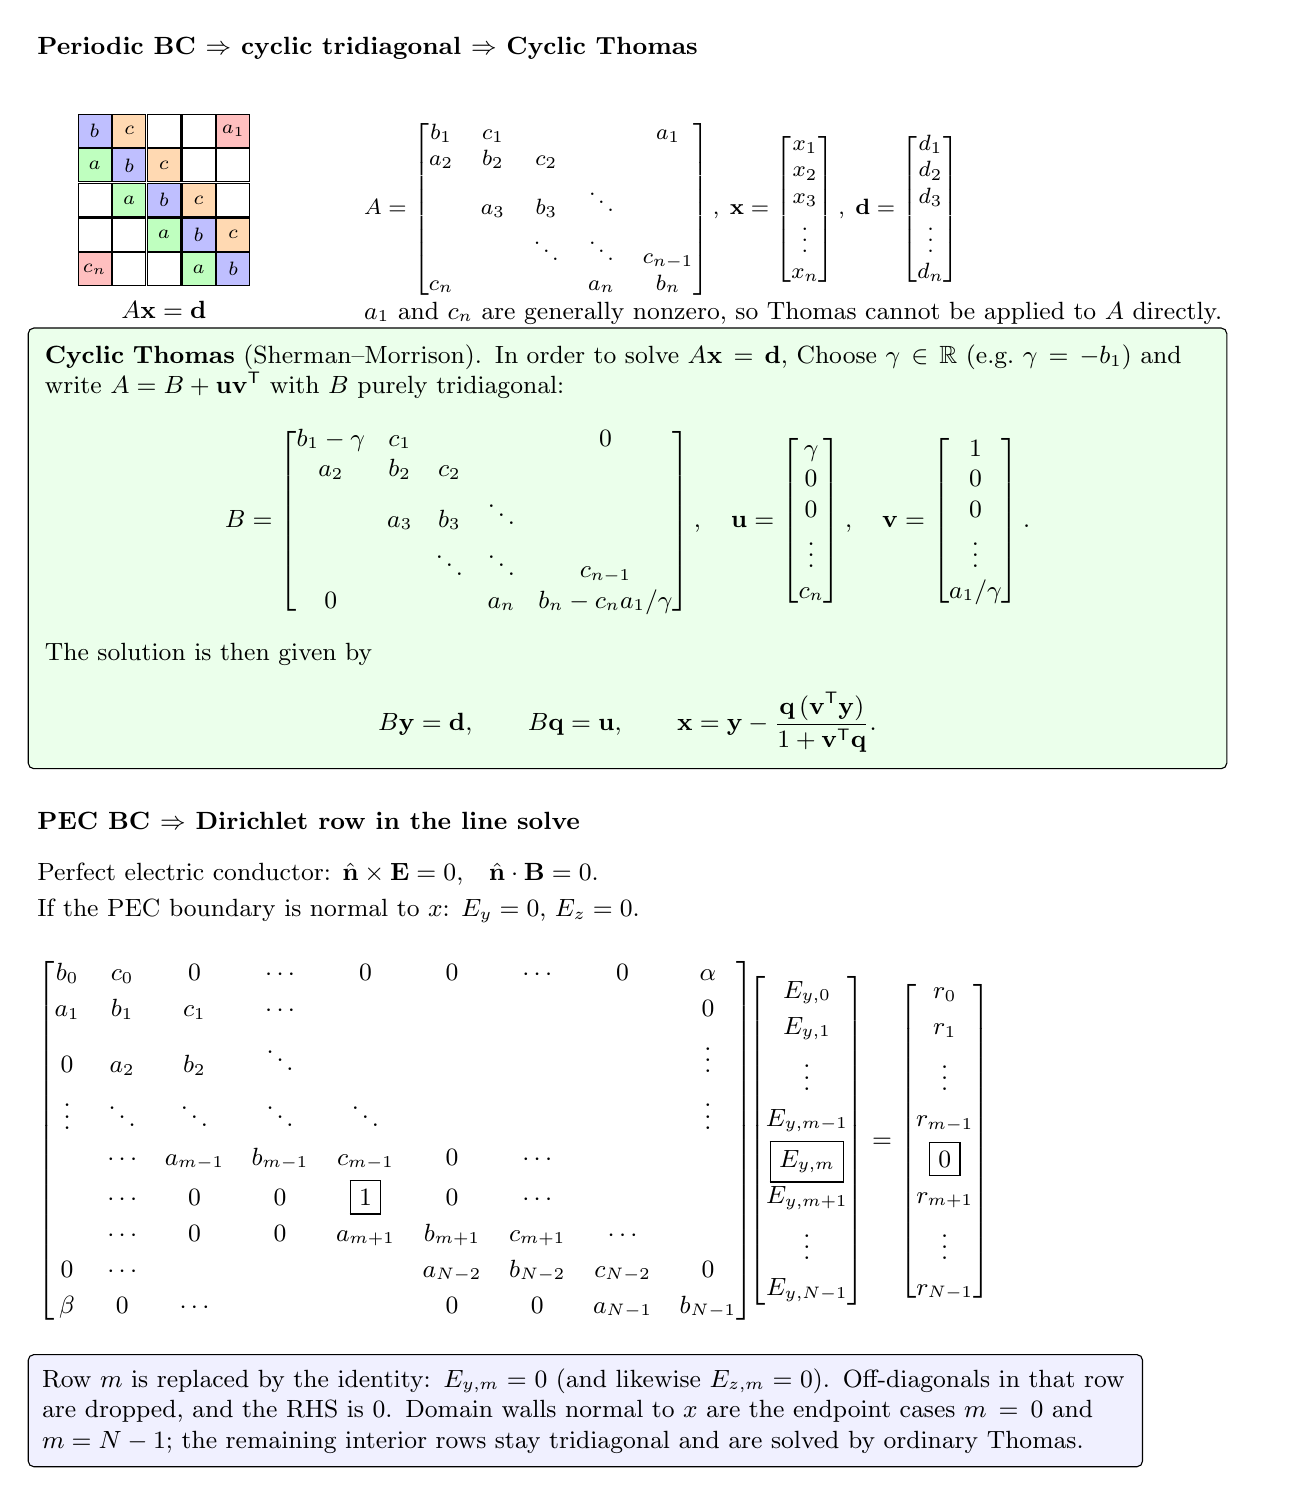
\begin{tikzpicture}[
    font=\small,
    >=Stealth,
    title/.style={font=\bfseries\small, anchor=west},
    tbox/.style={draw, rounded corners=2pt, align=left, inner sep=6pt, fill=green!8},
    pbox/.style={draw, rounded corners=2pt, align=left, inner sep=5pt, fill=blue!6, text width=13.8cm},
    cell/.style={draw, minimum size=0.42cm, inner sep=0pt, font=\scriptsize},
]
\node[title] (tper) at (0,0) {Periodic BC $\Rightarrow$ cyclic tridiagonal $\Rightarrow$ Cyclic Thomas};

% ---- cyclic 5x5 schematic ----
\def\s{0.44}
\coordinate (A0) at (0.85,-1.05);
\foreach \i in {0,1,2,3,4} {
    \foreach \j in {0,1,2,3,4} {
        \node[cell, fill=white] at ($(A0)+(\j*\s,-\i*\s)$) {};
    }
}
\foreach \i in {0,1,2,3,4} {
    \node[cell, fill=blue!25] at ($(A0)+(\i*\s,-\i*\s)$) {$b$};
}
\foreach \i in {0,1,2,3} {
    \node[cell, fill=orange!30] at ($(A0)+({(\i+1)*\s},-\i*\s)$) {$c$};
    \node[cell, fill=green!25] at ($(A0)+(\i*\s,{-(\i+1)*\s})$) {$a$};
}
\node[cell, fill=red!25] at ($(A0)+(4*\s,0)$) {$a_1$};
\node[cell, fill=red!25] at ($(A0)+(0,-4*\s)$) {$c_n$};

\node[below=8pt] (axd) at ($(A0)+(2*\s,-4*\s)$) {$A\mathbf{x}=\mathbf{d}$};

% ---- cyclic A, x, d ----
\node[anchor=west, font=\footnotesize] at (4.15,-2.05) {$
\displaystyle
A=
\begin{bmatrix}
b_1 & c_1 & & & a_1 \\
a_2 & b_2 & c_2 & & \\
 & a_3 & b_3 & \ddots & \\
 & & \ddots & \ddots & c_{n-1} \\
c_n & & & a_n & b_n
\end{bmatrix},\;
\mathbf{x}=
\begin{bmatrix} x_1 \\ x_2 \\ x_3 \\ \vdots \\ x_n \end{bmatrix},\;
\mathbf{d}=
\begin{bmatrix} d_1 \\ d_2 \\ d_3 \\ \vdots \\ d_n \end{bmatrix}
$};

\node[anchor=north west, text width=11.4cm] (noteA) at (4.15,-3.1) {
    $a_1$ and $c_n$ are generally nonzero, so Thomas cannot be applied to $A$ directly.
};

% ---- Sherman--Morrison box ----
\node[tbox, anchor=north west, text width=14.8cm] (ct) at (0,-3.55) {
    \textbf{Cyclic Thomas} (Sherman--Morrison).
    In order to solve $A\mathbf{x}=\mathbf{d}$,
    Choose $\gamma\in\mathbb{R}$ (e.g.\ $\gamma=-b_1$) and write $A=B+\mathbf{u}\mathbf{v}^{\mathsf{T}}$ with $B$ purely tridiagonal:
    \[
    \arraycolsep=4pt
    B=
    \begin{bmatrix}
    b_1-\gamma & c_1 & & & 0 \\
    a_2 & b_2 & c_2 & & \\
     & a_3 & b_3 & \ddots & \\
     & & \ddots & \ddots & c_{n-1} \\
    0 & & & a_n & b_n-c_n a_1/\gamma
    \end{bmatrix},
    \quad
    \mathbf{u}=
    \begin{bmatrix} \gamma \\ 0 \\ 0 \\ \vdots \\ c_n \end{bmatrix},
    \quad
    \mathbf{v}=
    \begin{bmatrix} 1 \\ 0 \\ 0 \\ \vdots \\ a_1/\gamma \end{bmatrix}.
    \]
    The solution is then given by
    \[
    B\mathbf{y}=\mathbf{d},\qquad B\mathbf{q}=\mathbf{u},
    \qquad
    \mathbf{x}
    =\mathbf{y}-\dfrac{\mathbf{q}\,(\mathbf{v}^{\mathsf{T}}\mathbf{y})}{1+\mathbf{v}^{\mathsf{T}}\mathbf{q}}.
    \]
};

% ========== PEC ==========
\node[title, anchor=north west] (tpec) at ($(ct.south west)+(0,-0.42)$)
    {PEC BC $\Rightarrow$ Dirichlet row in the line solve};

\node[anchor=north west, align=left] (pecintro) at ($(tpec.south west)+(0,-0.18)$) {
    Perfect electric conductor:
    $\hat{\mathbf{n}}\times\mathbf{E}=0$,\quad
    $\hat{\mathbf{n}}\cdot\mathbf{B}=0$.\\[2pt]
    If the PEC boundary is normal to $x$:
    $E_y=0$,\ $E_z=0$.
};

\node[anchor=north west] (pecmat) at ($(pecintro.south west)+(0,-0.22)$) {$
\displaystyle
\begin{bmatrix}
b_0 & c_0 & 0 & \cdots & 0 & 0 & \cdots & 0 & \alpha \\[2pt]
a_1 & b_1 & c_1 & \cdots & & & & & 0 \\[2pt]
0 & a_2 & b_2 & \ddots & & & & & \vdots \\[2pt]
\vdots & \ddots & \ddots & \ddots & \ddots & & & & \vdots \\[2pt]
 & \cdots & a_{m-1} & b_{m-1} & c_{m-1} & 0 & \cdots \\[2pt]
 & \cdots & 0 & 0 & \boxed{1} & 0 & \cdots \\[2pt]
 & \cdots & 0 & 0 & a_{m+1} & b_{m+1} & c_{m+1} & \cdots \\[2pt]
0 & \cdots & & & & a_{N-2} & b_{N-2} & c_{N-2} & 0 \\[2pt]
\beta & 0 & \cdots & & & 0 & 0 & a_{N-1} & b_{N-1}
\end{bmatrix}
\!\!
\begin{bmatrix}
E_{y,0}\\[2pt]
E_{y,1}\\[2pt]
\vdots\\[2pt]
E_{y,m-1}\\[2pt]
\boxed{E_{y,m}}\\[2pt]
E_{y,m+1}\\[2pt]
\vdots\\[2pt]
E_{y,N-1}
\end{bmatrix}
=
\begin{bmatrix}
r_0\\[2pt]
r_1\\[2pt]
\vdots\\[2pt]
r_{m-1}\\[2pt]
\boxed{0}\\[2pt]
r_{m+1}\\[2pt]
\vdots\\[2pt]
r_{N-1}
\end{bmatrix}
$};

\node[pbox, anchor=north west] at ($(pecmat.south west)+(0,-0.28)$) {
    Row $m$ is replaced by the identity:
    $E_{y,m}=0$ (and likewise $E_{z,m}=0$).
    Off-diagonals in that row are dropped, and the RHS is $0$.
    Domain walls normal to $x$ are the endpoint cases $m=0$ and $m=N-1$;
    the remaining interior rows stay tridiagonal and are solved by ordinary Thomas.
};
\end{tikzpicture}
\end{document}
